\subsubsection{Finite variance}\label{rectassumptionsvariance}

In the collision and messages plots we haven't trends but the behaviour is
blockwise, as we can see for example in \figref{fig:recttimevariance} with
swinging results and also in this case the order of magnitude of the residual is
lower than the one of the average predicted response, so we can conclude that
the assumption of finite variance is still valid.

As for other scenarios, to verify the assumption for the residuals of the 99th
percentile of the total broadcast time we need to perform a logarithmic
transformation of the predicted variable. The result is shown in
\figref{fig:recttimevariance}.

\begin{figure}[htb]
	\centering
	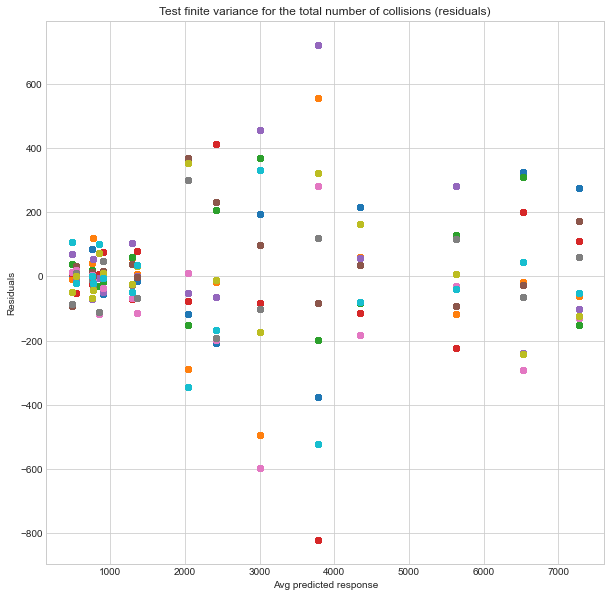
\includegraphics[width=0.37\textwidth]{img/rect/collisionvariance.png}
	\caption{Scatter plot of the variance of the residuals of the
	collisions. No trends but blockwise
	behaviour}\label{fig:recttimevariance}
\end{figure}

In order to meet the requirement of finite variance for the residuals of the
total broadcast time, as in other scenarios a transformed model is needed: \(y'
= \ln(y)\).
